\begin{figure}[!htbp]
\centering
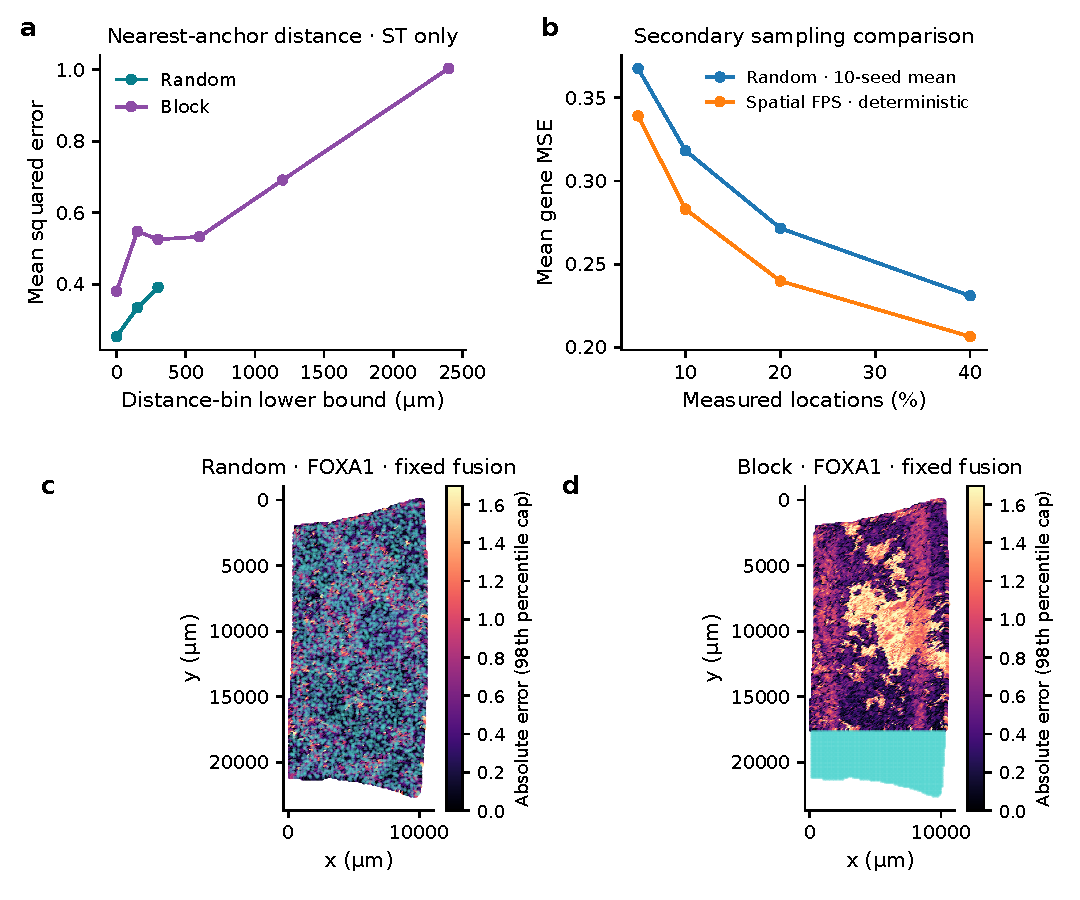
\includegraphics[width=\textwidth,height=0.60\textheight,keepaspectratio]{figures/Figure6.pdf}
\caption{\textbf{Spatial diagnostics reveal heterogeneous error beyond an overall prediction score.} Development results use TENX99 and the frozen 50-gene panel. \textbf{a,} Mean gene MSE versus nearest-anchor distance for molecular interpolation at 20\% coverage under distributed and development block masks; only occupied distance bins are shown. \textbf{b,} Development comparison of random and spatial farthest-point sampling, shown as MSE at matched measured-location budgets. These are descriptive single-patient sampling diagnostics, not a demonstration of universally optimal acquisition. \textbf{c,d,} Absolute-error maps for the preselected gene \textit{FOXA1}, fixed fusion, 20\% coverage and replicate 0 under random and block masks. Both maps use the same error scale, capped at the 98th percentile of the pooled preselected map-source values, which also include the archived capture-window condition; no locations are removed. Missing-region shape, available anchors and scored tissue differ between the maps. The figure illustrates why distance-bin support and spatial errors should accompany global correlation and why development geometry findings require independent evaluation.}
\label{fig:geometry}
\end{figure}
